% vim: ft=tex
\chapter{Requirements}
The requirements gathered during the first and second meeting with the client are
explained in this chapter. These are more concrete than the ones listed in the
Task Description in \autoref{ch:task-desc}.

First of all, these are the client's priorities:

\begin{enumerate}
\item Federation functionality, namely:
	\begin{enumerate}
		\item Topology definition
		\item DIM synchronization
		\item Message routing
	\end{enumerate}
\item \Gls{HA}
\item Persistence synchronization
\item Encryption (optional)
\item DIM access control
\item OPC UA \gls{HA} (optional)
\end{enumerate}

The following sections explain the requirements in greater detail.

\section{Functional}
This section elucidates the functional requirements, as opposed to the
non-functional requirements.

\subsection{Federation}
Roadster will need to be run on multiple nodes in a hierarchical topology,
forming a distributed computing architecture. The root node would then act as
the client-facing server. Typical node topologies include:

\begin{description}
	\item [ Single level, single node ] \hfill\\
		This is the legacy setup and is what Roadster is already able
		to do. It consists of a single node. This is illustrated in
		\autoref{fig:topo:sl:noha}.

	\item [ Multi level ] \hfill\\
		This is the most basic federation setup. There is a root node, and
		two subnodes. Each subnode is directly connected to a field device such as a
		PLC or an emergency phone. This is illustrated in
		\autoref{fig:topo:ml:noha}.
\end{description}

\begin{figure}[]
	\center
	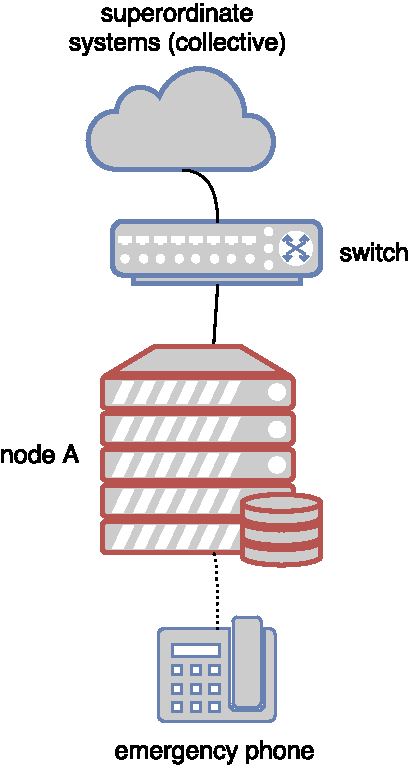
\includegraphics[width=0.25\textwidth]{img/topo_sl_noha.pdf}
	\caption{Physical legacy example: a single node and a field device each}
	\label{fig:topo:sl:noha}
\end{figure}
\begin{figure}[]
	\center
	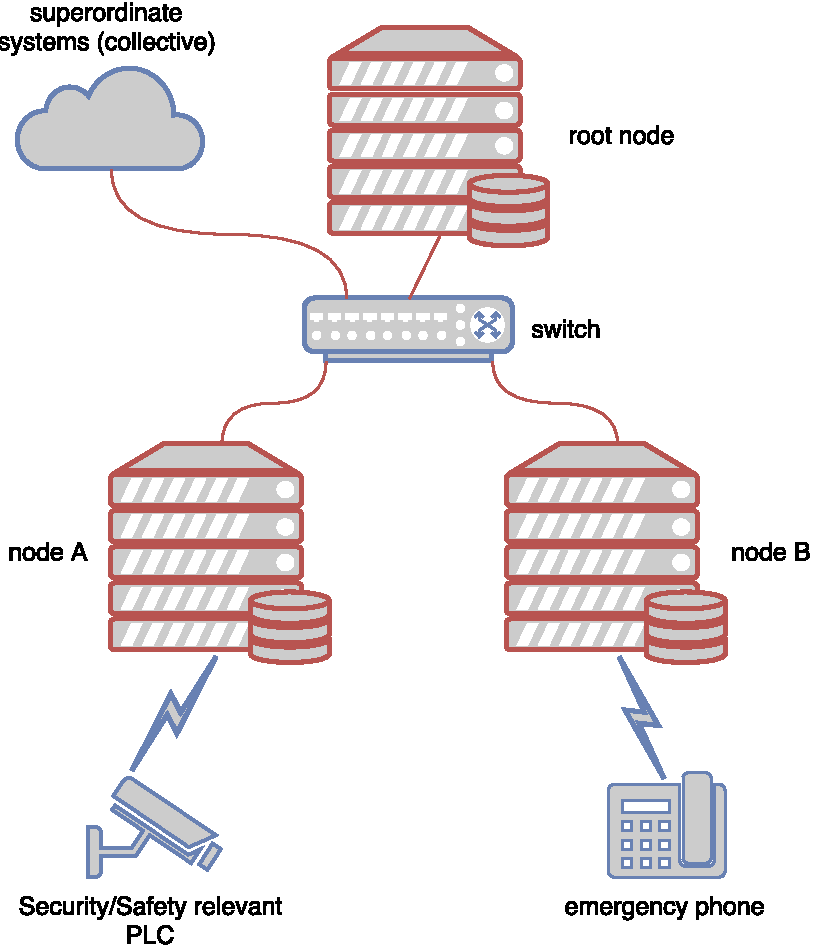
\includegraphics[width=0.5\textwidth]{img/topo_ml_noha.pdf}
	\caption{Physical federation topology example: supernode, two subnodes, a field device each}
	\label{fig:topo:ml:noha}
\end{figure}

This is formally specified in \autoref{lst:feature:federation}

\begin{listing}
	\inputminted{Gherkin}{listings/features/federation/federation.feature}
	\caption{Formal federation feature}
	\label{lst:feature:federation}
\end{listing}

\subsubsection{DIM extension}

\paragraph{Synchronization}
% TODO: it needs to go both ways!
Extending the \gls{CSP} to keep the \gls{DIM} in sync across all nodes is a central
part of the federation functionality. This means replicating modifications to
the dynamic DIM objects to all other actors on the node (legacy behavior) and
to all other nodes.

According to the meta model in \autoref{fig:roadster:meta-model}, these dynamic
objects are exactly the instances of one of the following three
classes (marked yellow in the class diagram):
\begin{itemize}
	\item \rb{DataItem}
	\item \rb{Session}
	\item \rb{Case}
\end{itemize}

As described earlier, instances of these entity classes are marked "dirty" when
modified until they are replicated.

\paragraph{Access control}
The above requirements imply that changes to the \gls{DIM} can only be done by the
respective node. In other words, a node can only change objects owned by itself. It
cannot change objects of other nodes directly. This is to ensure that each node is its own source of truth
to all other nodes in the setup. Only the responsible node can enforce a single
sequence of updates to its part of the DIM, which is necessary to guarantee
consistency \cite[Chapter 5, Reliable Pub-Sub (Clone Pattern), Republishing
Updates from Clients]{zmq:zguide}.

These two aspects to the DIM extension are formally specified in \autoref{lst:feature:federation:dimsync}

\begin{listing}
	\inputminted{Gherkin}{listings/features/federation/dim_extension.feature}
	\caption{Formal DIM synchronization feature}
	\label{lst:feature:federation:dimsync}
\end{listing}

\subsubsection{Autonomy}
It's important that every node subtree can keep up the operation autonomously even if the
link to its supernode fails or the supernode itself fails. This means that updates to
the \gls{DIM} are allowed even when the supernode is unavailable. After the
recovery from the outage, the \gls{DIM} synchronization shall be reinitiated so
all pending updates are shared to all other nodes (through the supernode).

This is formally specified in \autoref{lst:feature:federation:autonomy}

\begin{listing}
	\inputminted{Gherkin}{listings/features/federation/autonomy.feature}
	\caption{Formal autonomy feature}
	\label{lst:feature:federation:autonomy}
\end{listing}

\subsubsection{Message routing}
There needs to be a message routing mechanism so a user
of one node's web UI can send a command (passed as a message) to another node where it will be
executed. An example for this is a forced value in the DIM to ignore the
actually measured value reported by a device in case the device is known to be
wrong. The common case where the command is issued at a higher level in the node
topology is priority. E.g. in a setup with a root node and two
subnodes A and B, issuing a command on A for B has a low priority.

This is formally specified in \autoref{lst:feature:federation:cmdrouting}

\begin{listing}
	\inputminted{Gherkin}{listings/features/federation/message_routing.feature}
	\caption{Formal message routing feature}
	\label{lst:feature:federation:cmdrouting}
\end{listing}

\subsection{High availability}
Roadster must be able to run in certain high availability setups. Achieving
this is done by adding redundant Roadster nodes.

The following additional federation topologies must be supported:
\begin{description}
	\item [ Single level \gls{HA} ] \hfill\\
		This is when there are exactly two nodes, both of them
		connected to the same PLC. There are two nodes for redundancy. This is illustrated in
		\autoref{fig:topo:sl:ha}.

	\item [ Multi level, \gls{HA} at root only ] \hfill\\
		There can be multiple levels in the hierarchy, such as two or
		three (anything else is considered exotic), and there's a HA
		cluster at the root. An example of this setup is illustrated in
		\autoref{fig:topo:ml:ha}.
\end{description}

\begin{figure}[]
	\center
	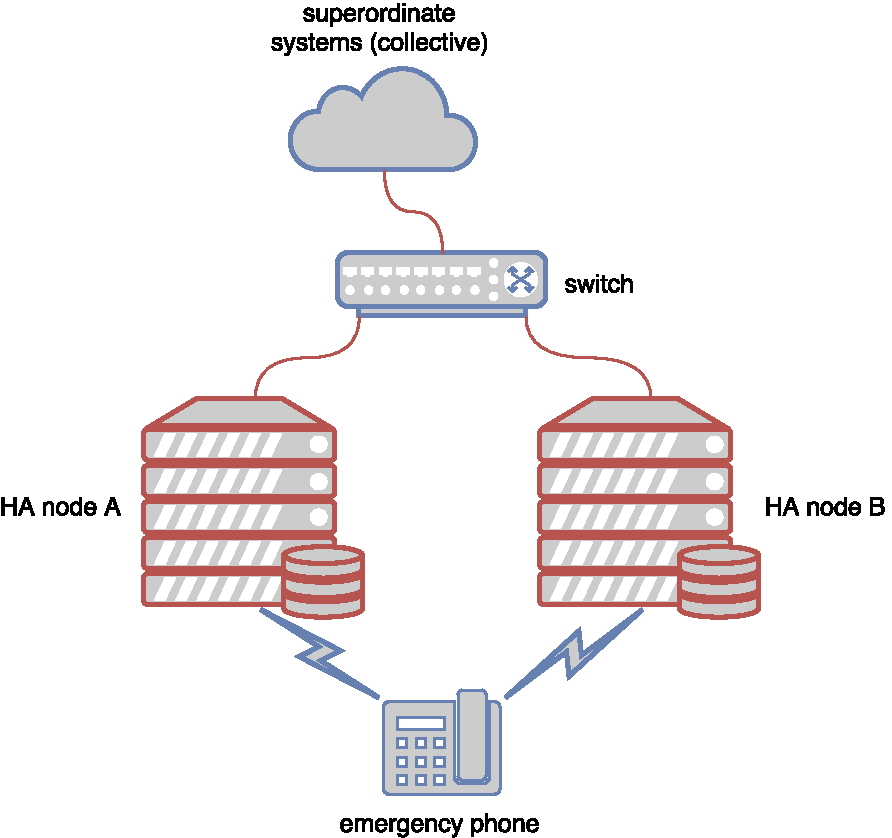
\includegraphics[width=0.5\textwidth]{img/topo_sl_ha.pdf}
	% TODO: update illustration to include multiple field devices
	\caption{Federation example: a HA cluster and redundantly connected field devices}
	\label{fig:topo:sl:ha}
\end{figure}
\begin{figure}[]
	\center
	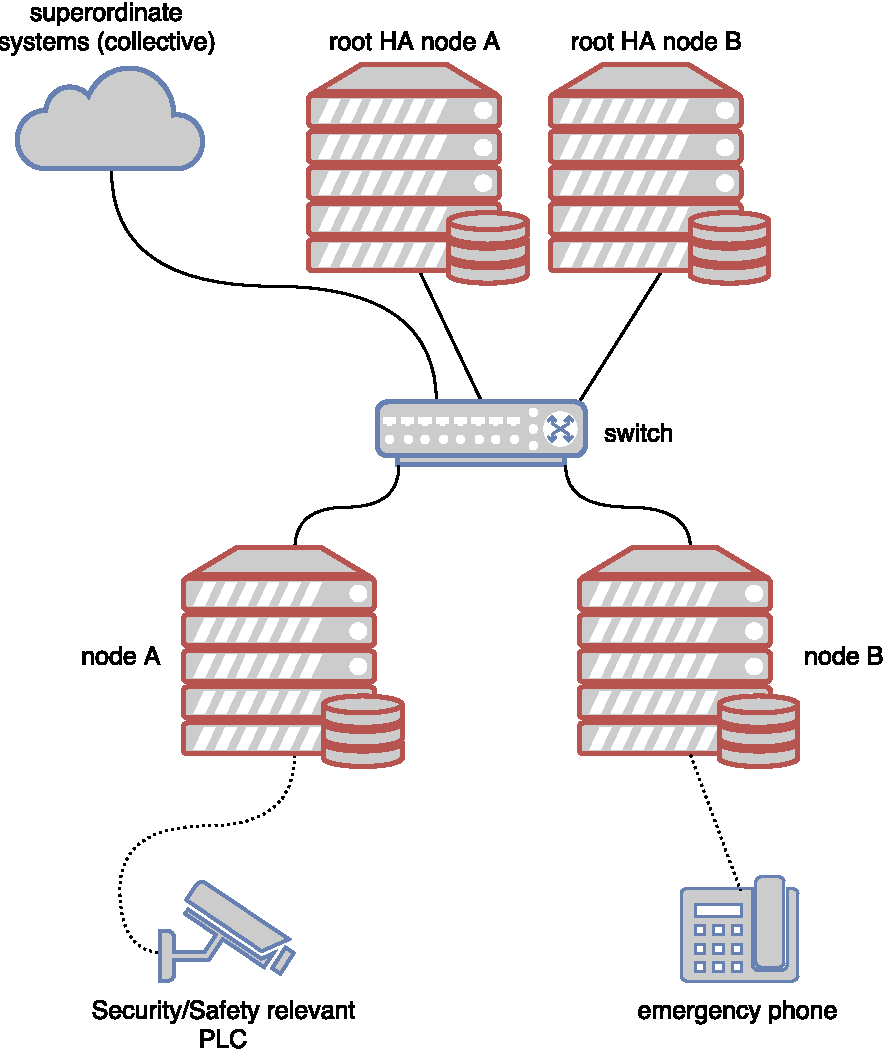
\includegraphics[width=0.5\textwidth]{img/topo_ml_ha.pdf}
	% TODO: update illustration to include multiple field devices
	\caption{Federation example: HA cluster at root, two subnodes, each with field devices}
	\label{fig:topo:ml:ha}
\end{figure}

The following exotic cases can be ignored: % FIXME

\begin{description}
	\item [ Multi level, \gls{HA} at bottom ] \hfill\\
	A single root node at the top and a subordinate HA pair each connected
	to the same field device.

	\item [ Multi level, \gls{HA} in the middle ] \hfill\\
	A single root node at the top, a subordinate HA pair, which in turn has
	a subordinate node connected to some field device.
\end{description}

The following sections contain the concrete requirements about the two
different \gls{HA} levels.

% TODO: unify with ML
\subsubsection{Single level}
This is where each of the two nodes forming a HA unit is directly connected to a number of
subsystems such as \glspl{PLC}, forming two redundant network paths to each
subsystem. Both nodes are able to interact with the subsystems to perform
operation tasks (e.g. reading sensor data, writing down configurations), but
only one of them (the active one) must do so.

The two nodes must automatically find consensus on which one is currently active. The
passive one must automatically take over in case the active one is confirmed to
be dead.
\begin{itemize}
	\item Hardware/software failure on the primary node % TODO split
	\item Failure of one of the redundant networking paths connecting the subsystem to the two nodes % FIXME
\end{itemize}

\subsubsection{Multi level HA}
This is where a node pair is the parent of one or more subnodes.

The types of failures that need to be handled include:
\begin{itemize}
	\item Software failure on the primary node, like an application or OS crash
	\item Hardware failure on the primary node, like a defect power supply
	\item Failure of the network link connecting a node to the cluster
\end{itemize}

All three failure types listed above can collectively be called \emph{crash},
as their effects are the same from the point of view of the whole federation.

\subsection{Persistence synchronization}
This is about the synchronization of persisted data, which is currently stored
in \gls{tc} databases on a Roadster node. With the federation functionality, this is
still true: Every node will have its own key-value store. Updates for persisted
data must only flow from south to north (towards the root node), so the root
node can collect and maintain a replication of the persisted data of all
subnodes, recursively.

It's important that every node and its subnodes form an autonomous subtree. So
in case the link to its supernode fails, it has to continue working. As soon as
the link is repaired, synchronization of the delta (the newly added data) can
be initiatd. Sending just the delta should be possible since keys in the
database contain timestamps.

This is not the same as \gls{CHP} (\gls{DIM} synchronization), as the DIM is shared across
all nodes and is a relatively small data structure. The \gls{tc} databases
can possibly contain large amounts of data (in the hundreds of megabytes) and
are shared only towards the root node (thus "bubbling up").

100\% consistency is not an absolute requirement for persistence synchronization.
However, it is mandatory that updates make it to the root node within 30 seconds.

% ---------------------------------------------------------------------------
\section{Non-functional requirements}
The following subsections illustrate the non-functional requirements.

\subsection{Simplicity}
The two reoccuring patterns that surfaced during the requirements gathering
meeting were:

\begin{enumerate}
\item \gls{KISS} principle. Simplicity is favored, as experience shows that
	simpler systems are more stable, so complexity should be avoided if not
	absolutely necessary.

\item No premature optimization since it's the root of all evil.\footnote{Quote
	by Donald Knuth: ``Premature optimization is the root of all evil.''}
\end{enumerate}


\subsection{Testing}
Regarding testing, the following requirements exist:
\begin{itemize}
	\item the student's contributions are verified with unit tests
	\item use cases shall be integration tested in a close-to-reality setup, either automatically or manually
\end{itemize}

\subsection{High availability for OPC UA}
The high availability feature shall be design with \gls{opc-ua} in mind. It
should be easy to adapt it to the various kinds of server redundancy specified
in OPC-UA, including the transparent and non-transparent variants.

\subsection{Encryption}
\emph{This is optional. Also, this requirement has the lowest priority not
because it's insignificant, but because it's easy to enable transport level
security on \zmq sockets later on.}

The inter-node communication of a Roadster federation must be secured using
encryption. \zmq offers modern, authenticated encryption and performs server authentication at a minimum if when transport security is
enabled. Client authentication is favored, but not an absolute requirement.

\subsection{Coding Guidelines}
The coding guidelines desired by the client are basically the ones written down
in the popular Ruby style guide \cite{rb:style-guide}, with the following
differences or special remarks:

\begin{itemize}
	\item method calls: only use parenthesis when needed, even with arguments (as opposed to \footnote{\url{https://github.com/bbatsov/ruby-style-guide\#method-invocation-parens}})
	\item 2 blank lines before method definition (slightly extending \footnote{\url{https://github.com/bbatsov/ruby-style-guide\#empty-lines-between-methods}})
	\item YARD API doc, 1 blank comment line before param documentation, one blank comment line before code (ignoring \footnote{\url{https://github.com/bbatsov/ruby-style-guide\#rdoc-conventions}})
	\item Ruby 1.9 symbol keys are wanted (e.g. \rb{foo: "bar", baz: 42} instead of \rb{:foo => "bar", :baz => 42}, just like \footnote{\url{https://github.com/bbatsov/ruby-style-guide\#hash-literals}})
	\item align multiple assignments so there's a column of equal signs
\end{itemize}
